%%%%%%%%%%%%%%%%%%%%%%%%%%%%%%%%%%%%%%%%%%%%%%%%%%%%%%%%%%%%%%%%%%%%%%%%%%%%%%%%%%%%%
\clearpage
\section{Structure factors for Yukawa like potentials}~\\
\label{sect:SQ4Yukawa}
For charged colloidal dispersions analytical structure factors have been found in the mean spherical approximation \cite{Hayter1981,Hansen1982,Liu2005}. The hard core Yukawa potential (also called a screened Coulomb potential) is defined as
\begin{align}
u^\mathrm{Y}(r,K,Z) &= k_BT \begin{cases}
                             \infty, & \mbox{if } 0\leq r < \sigma \\
                             -\frac{K}{r/\sigma}\exp(-Z (r/\sigma-1)), & r\leq \sigma.
                            \end{cases}
\end{align}
In the limit of no screening, i.e. $Z=0$ the interaction is a purely Coloumb interaction proportional to $1/r$.

\subsection{Hard core double Yukawa interaction}~\\
\label{sect:SQ4doubleYukawa}
To describe a short range attractive and long range repulsive interaction Liu et al.\ \cite{Liu2005} calculated an analytical solution of Ornstein-Zernike equation in the mean spherical approximation. They assumed a potential of the form
\begin{align}\label{eq:SQ2Ypotential}
\frac{u^\mathrm{2Y}(r,\ldots)}{k_BT} &= \begin{cases}
                             \infty, & \mbox{if }  r < \sigma \\
                             -K_1\frac{\exp\left(-Z_1 \left(\frac{r}{\sigma}-1\right)\right)}{r/\sigma} -K_2\frac{\exp\left(-Z_2 \left(\frac{r}{\sigma}-1\right)\right)}{r/\sigma}, & r\leq \sigma.
                            \end{cases}
\end{align}
\begin{figure}[htb]
\captionsetup[subfigure]{position=b}
\centering
\subcaptionbox{Hard-core two-Yukawa potential \label{fig:2Yukawa_U} }{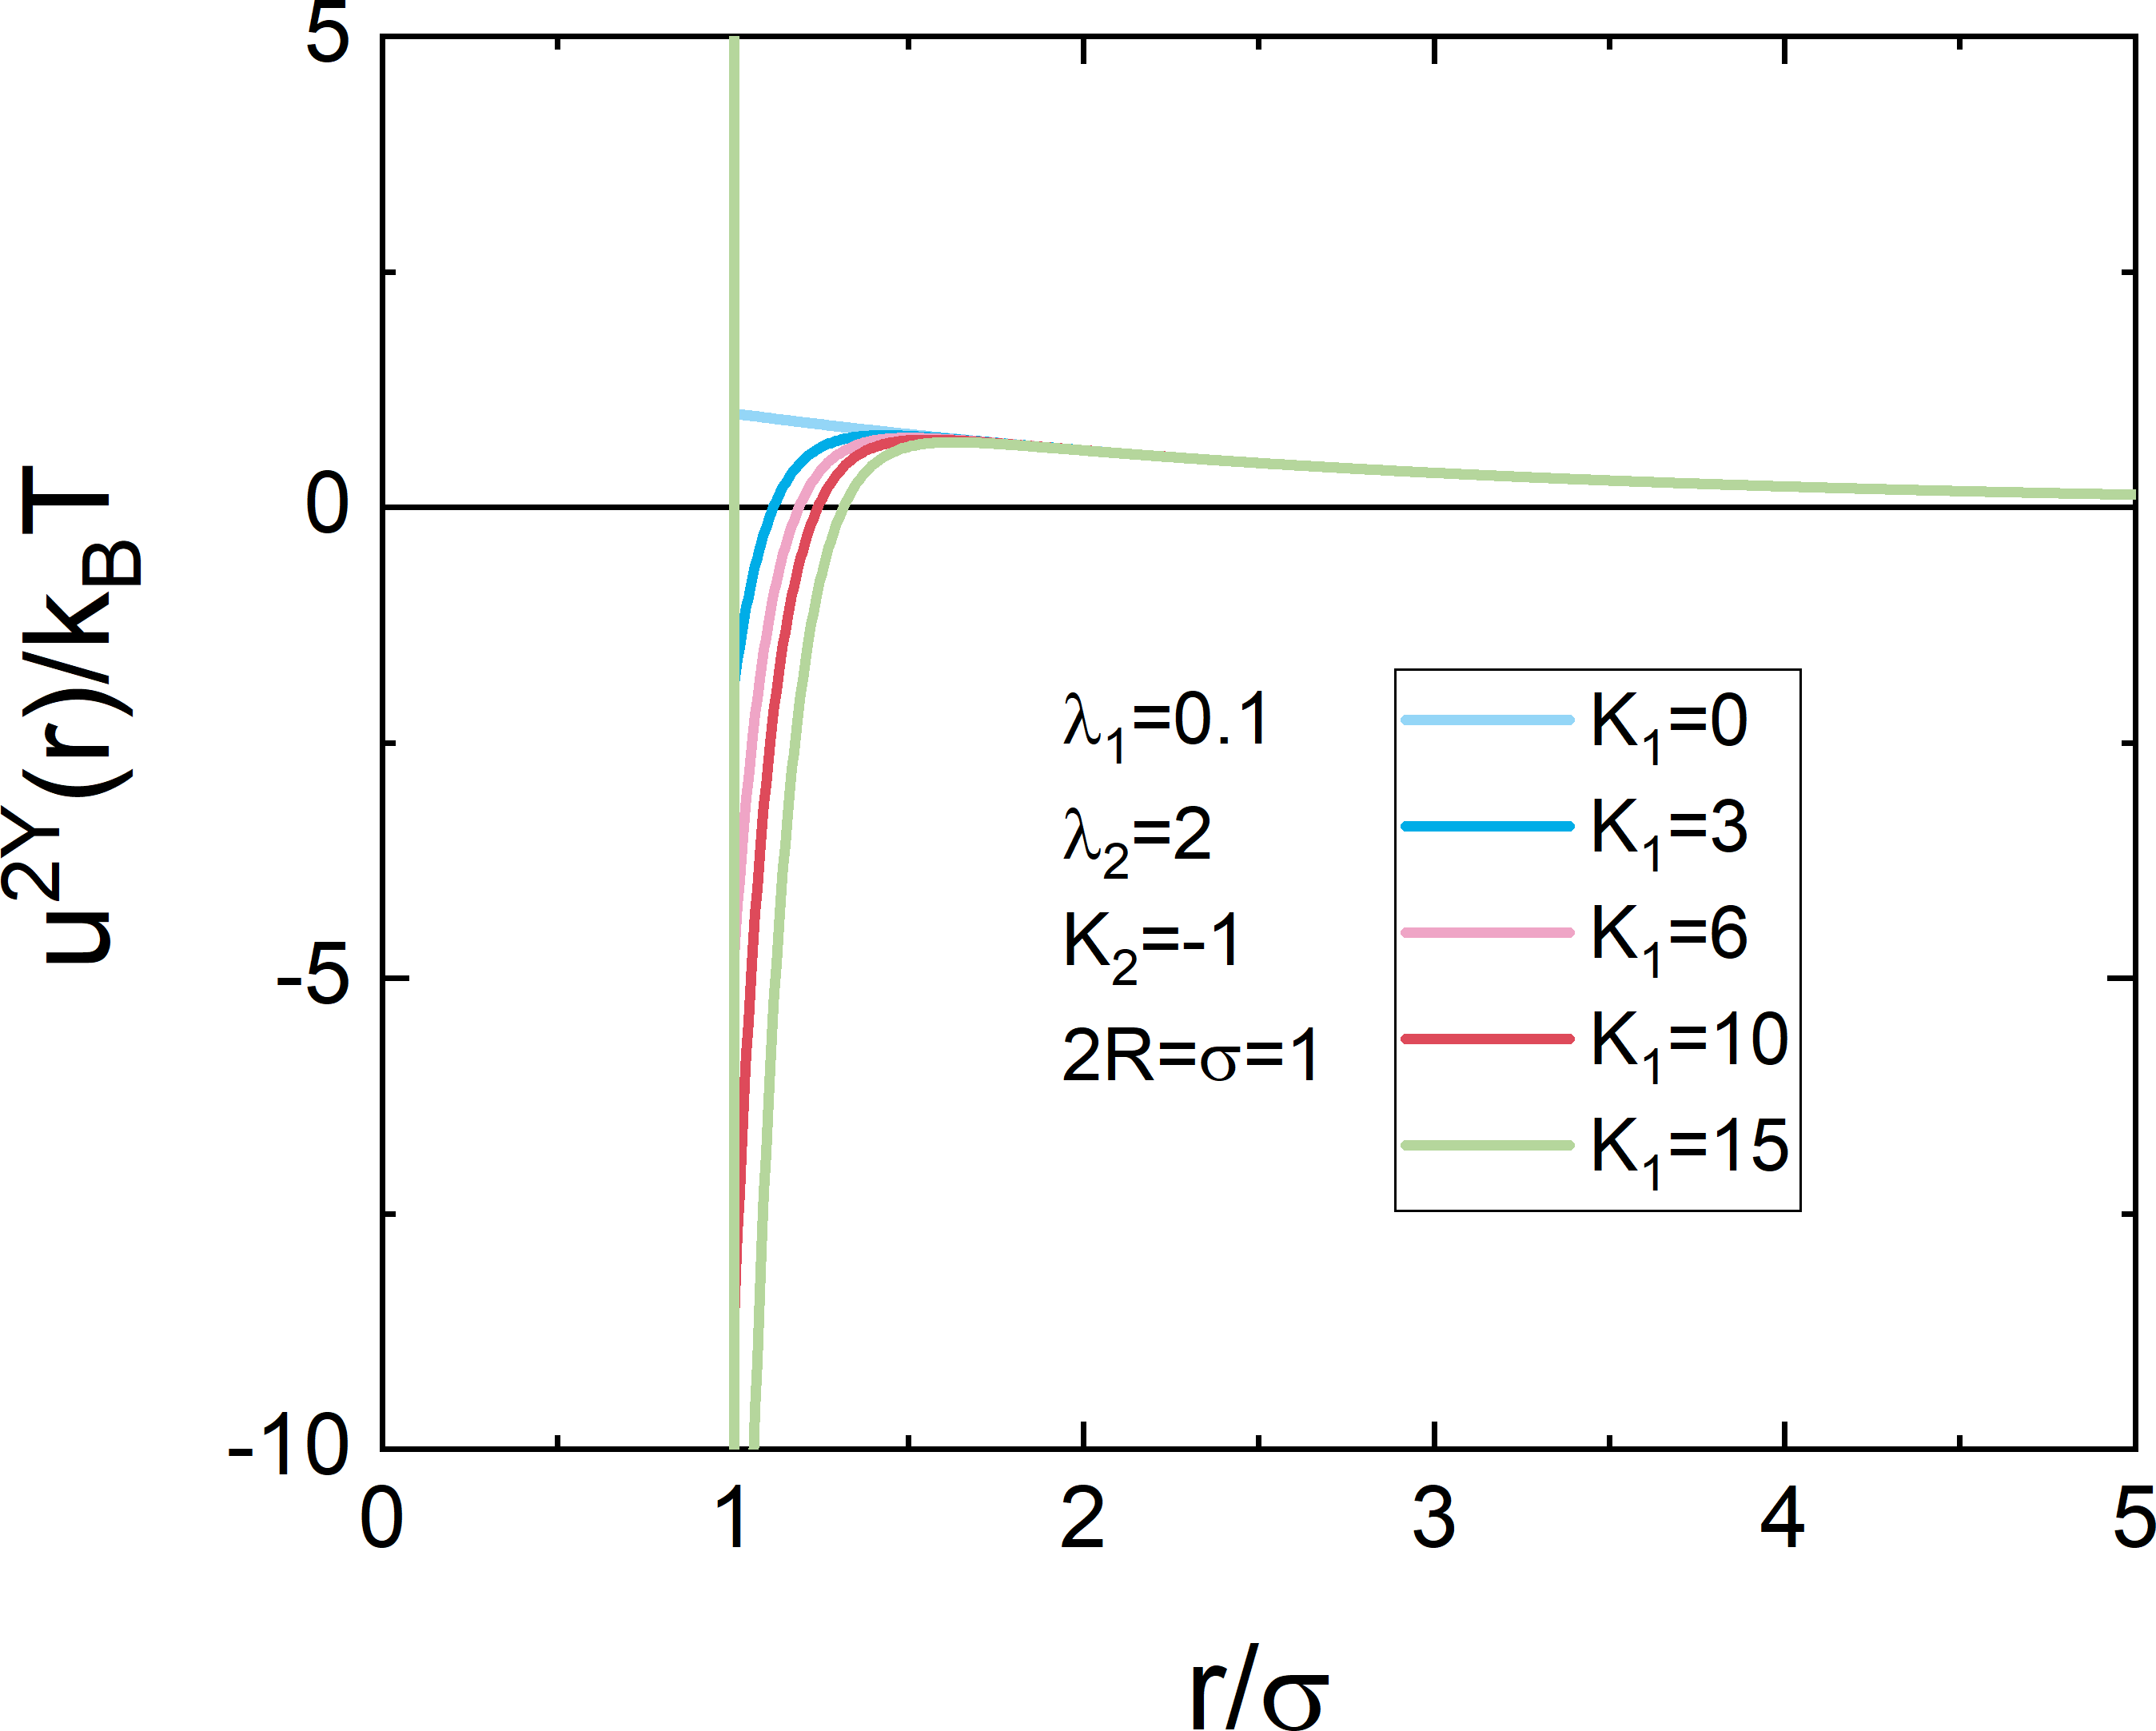
\includegraphics[width=0.45\textwidth]{../images/structure_factor/YukawaLike/TwoYukawaPotential.png}}
\hfill
\subcaptionbox{Mayer-f function of $\frac{u^\mathrm{2Y}(r,\ldots)}{k_BT}$. \label{fig:2YukawaMayerF} }{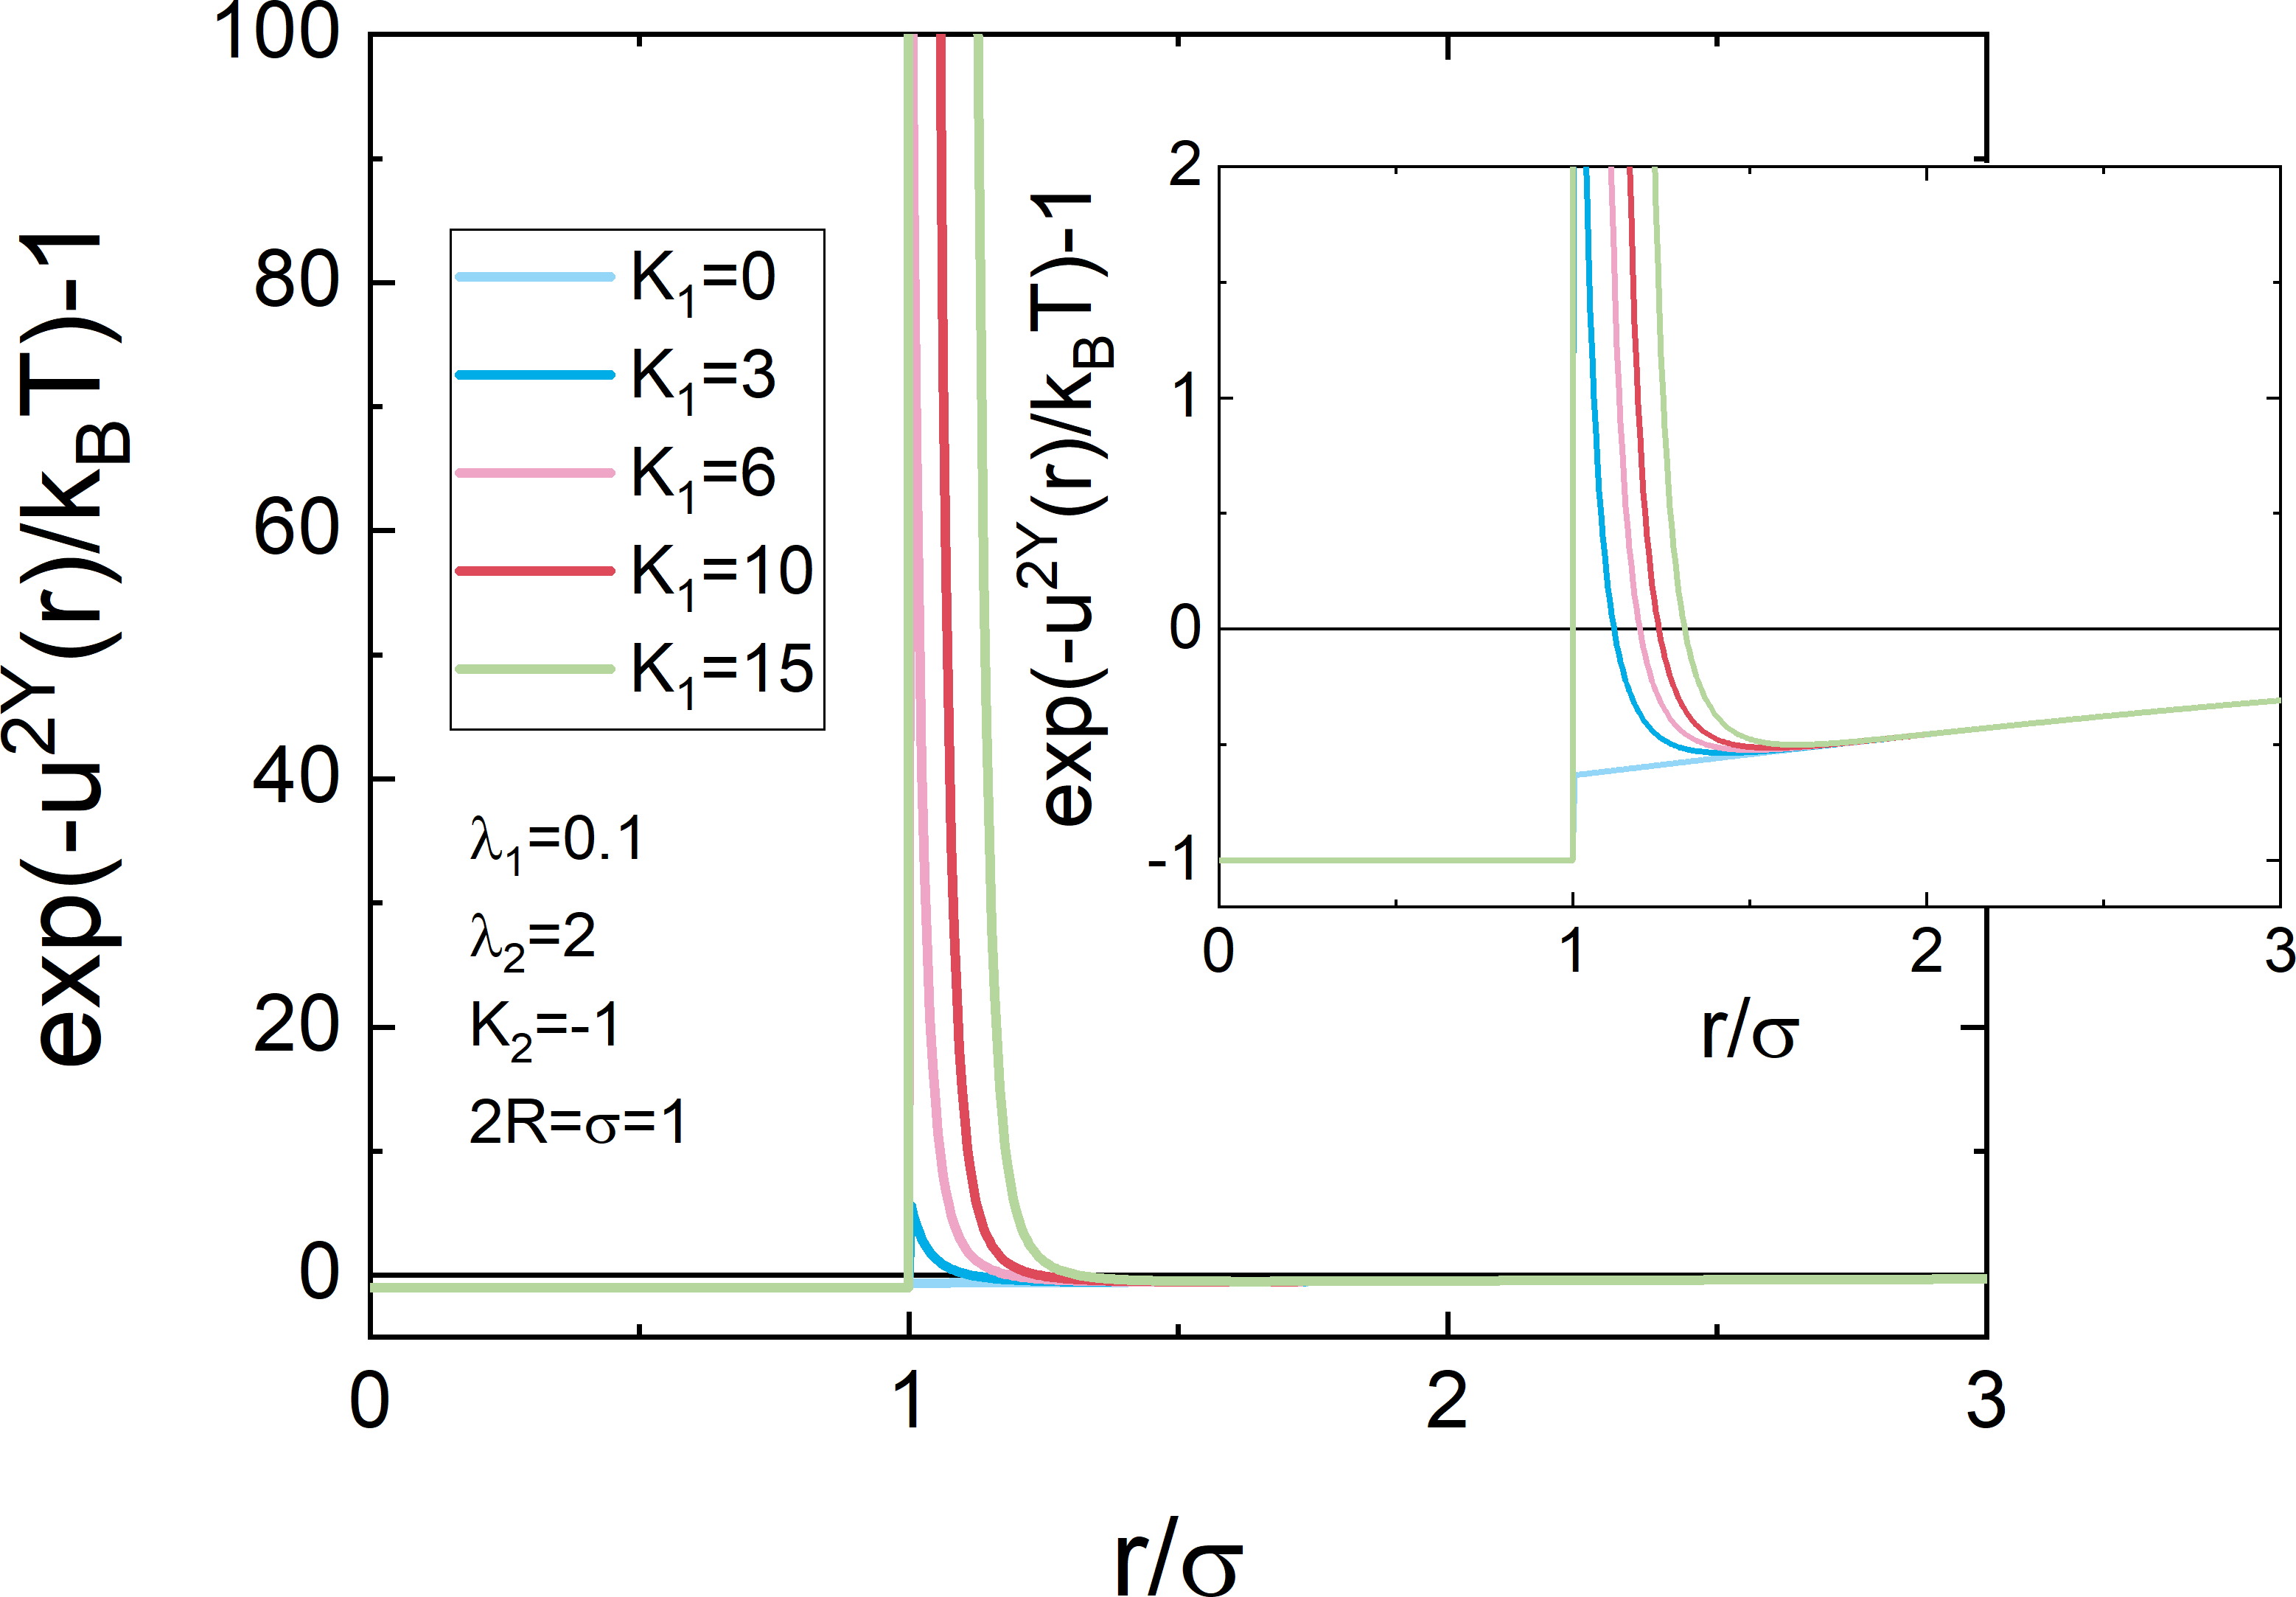
\includegraphics[width=0.53\textwidth]{../images/structure_factor/YukawaLike/TwoYukawaMayerf.png}}
\caption{Potential and corresponding Mayer-f function }
\label{fig:YukawaPot}
\end{figure}

\begin{figure}[htb]
\captionsetup[subfigure]{position=b}
\centering
\subcaptionbox{Structure factor of two-Yukawa potential in the mean spherical approximation showing a cluster peak. \label{fig:2YukawaSQ} }{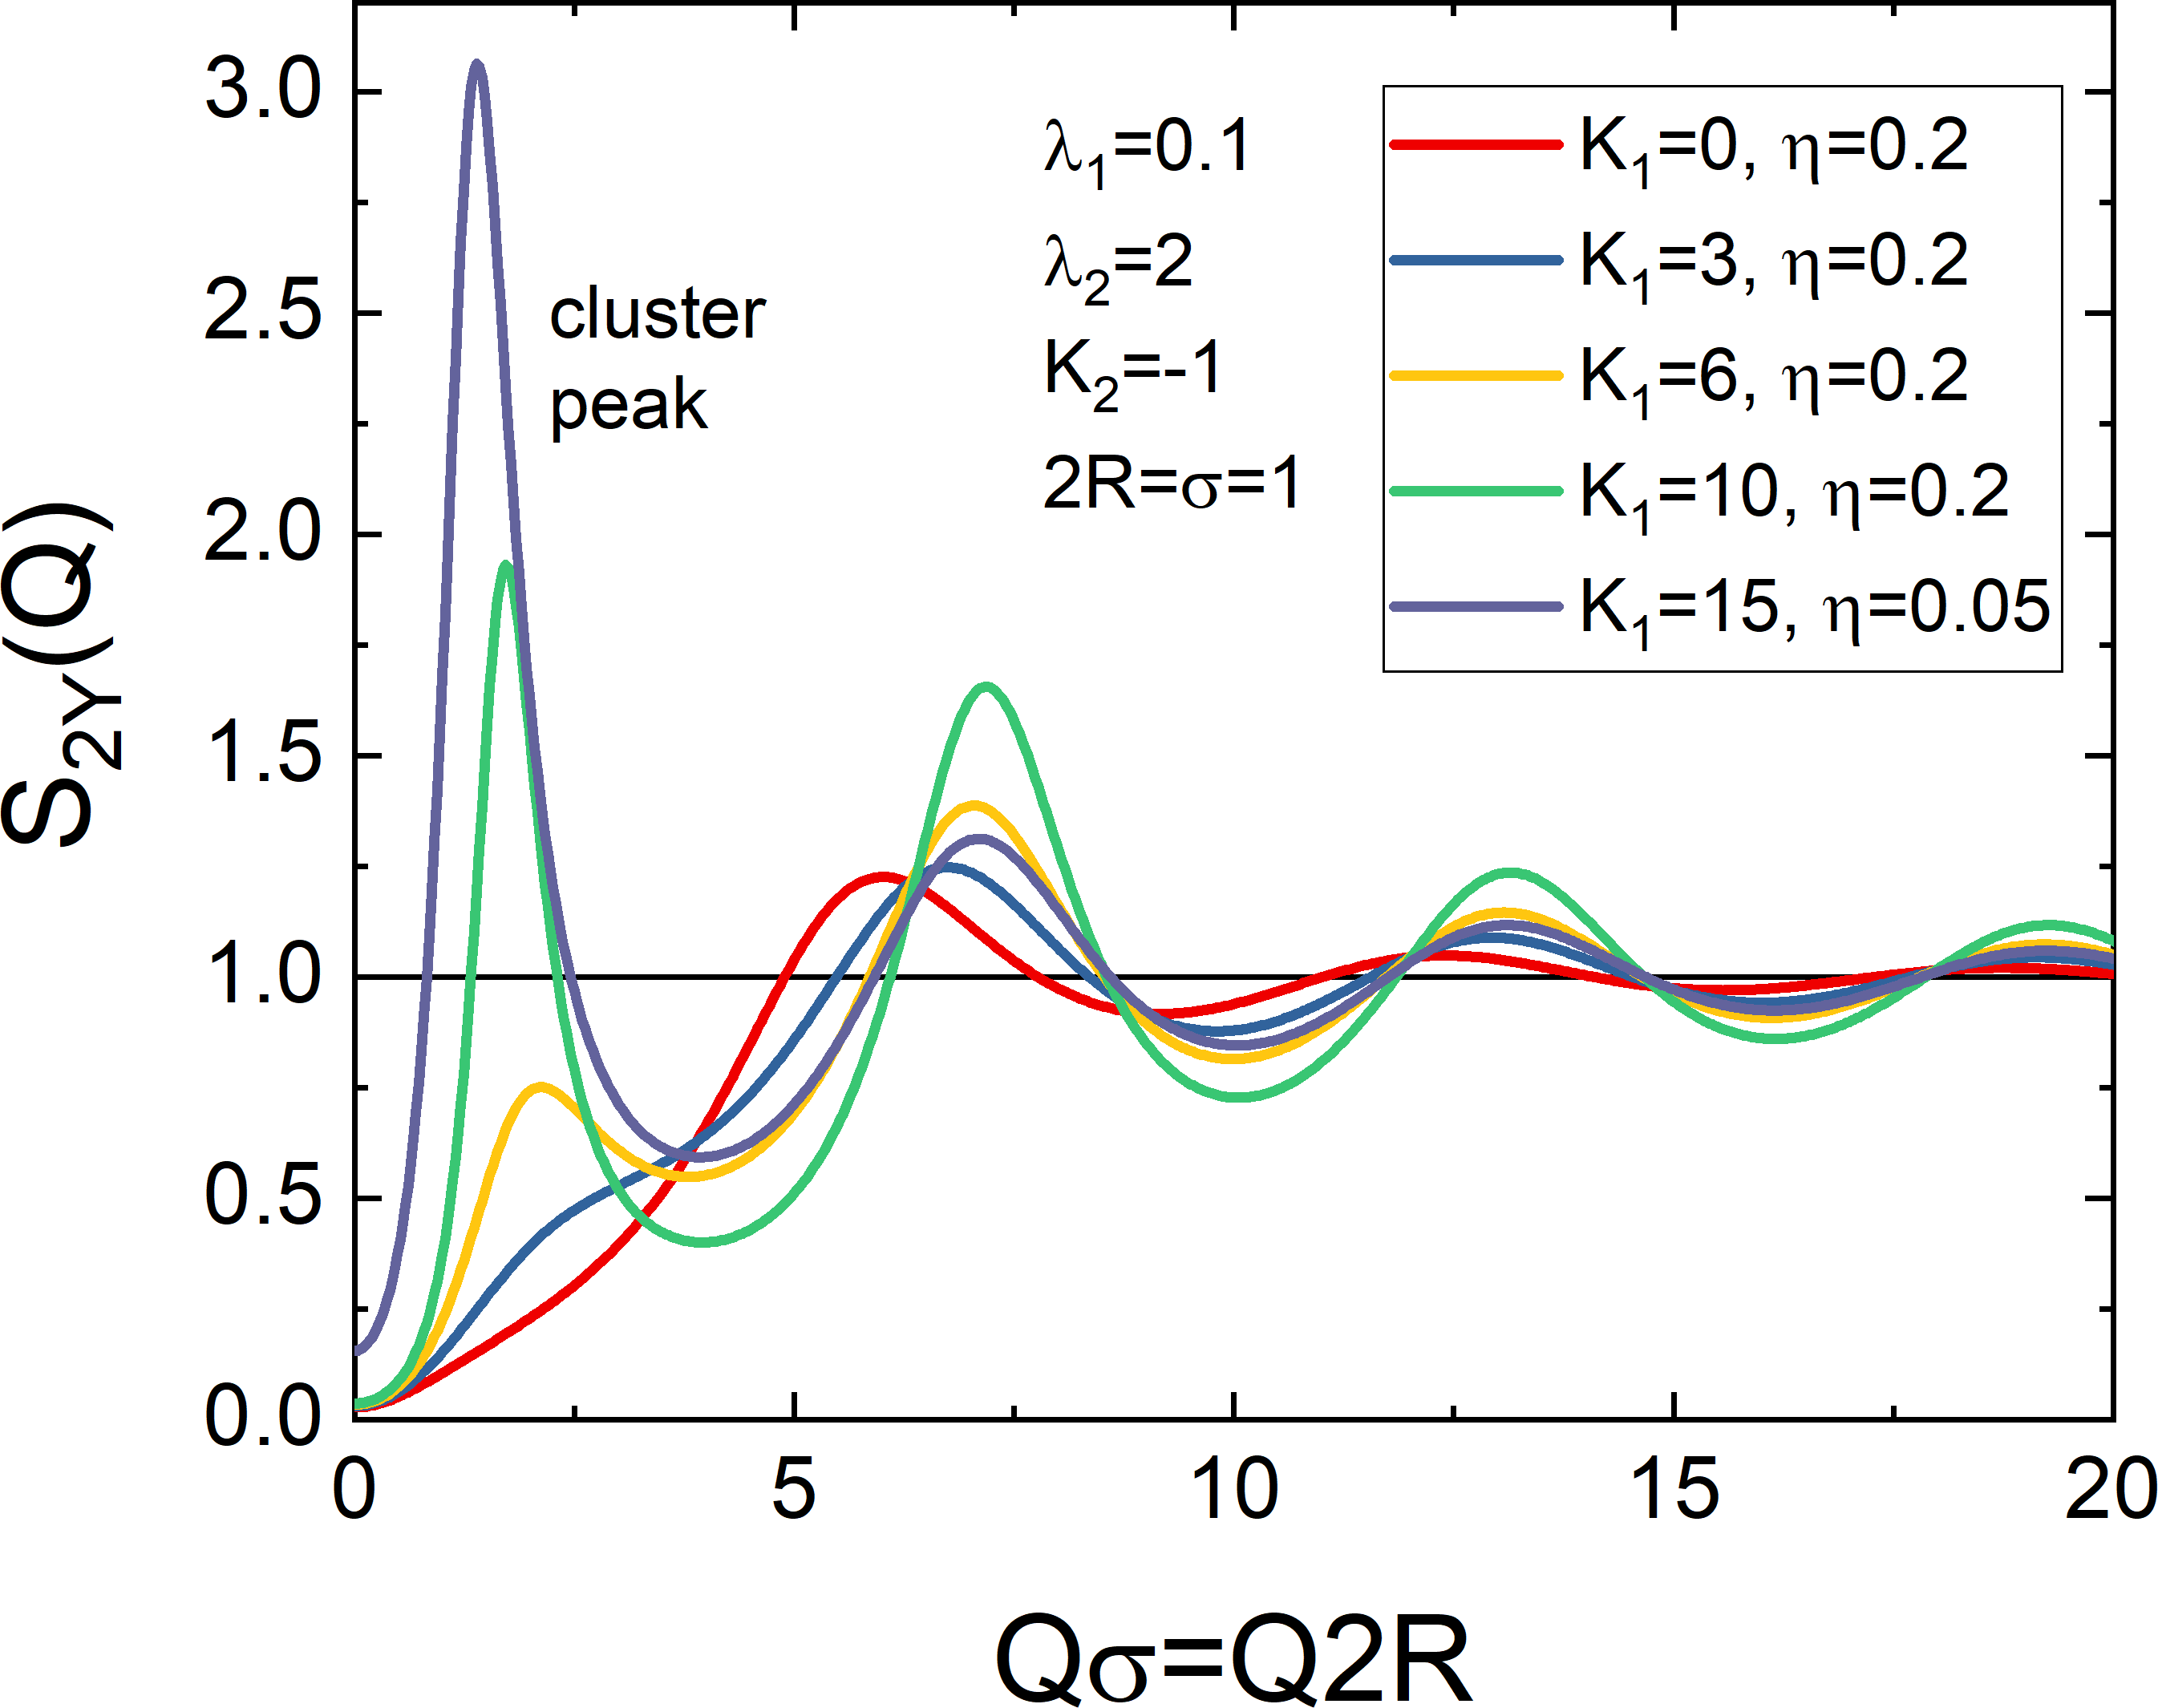
\includegraphics[width=0.48\textwidth]{../images/structure_factor/YukawaLike/TwoYukawa.png}}
\hfill
\subcaptionbox{Corresponding radial distribution function $g(r)$ to the structure factor on the left. \label{fig:2YukawaGR} }{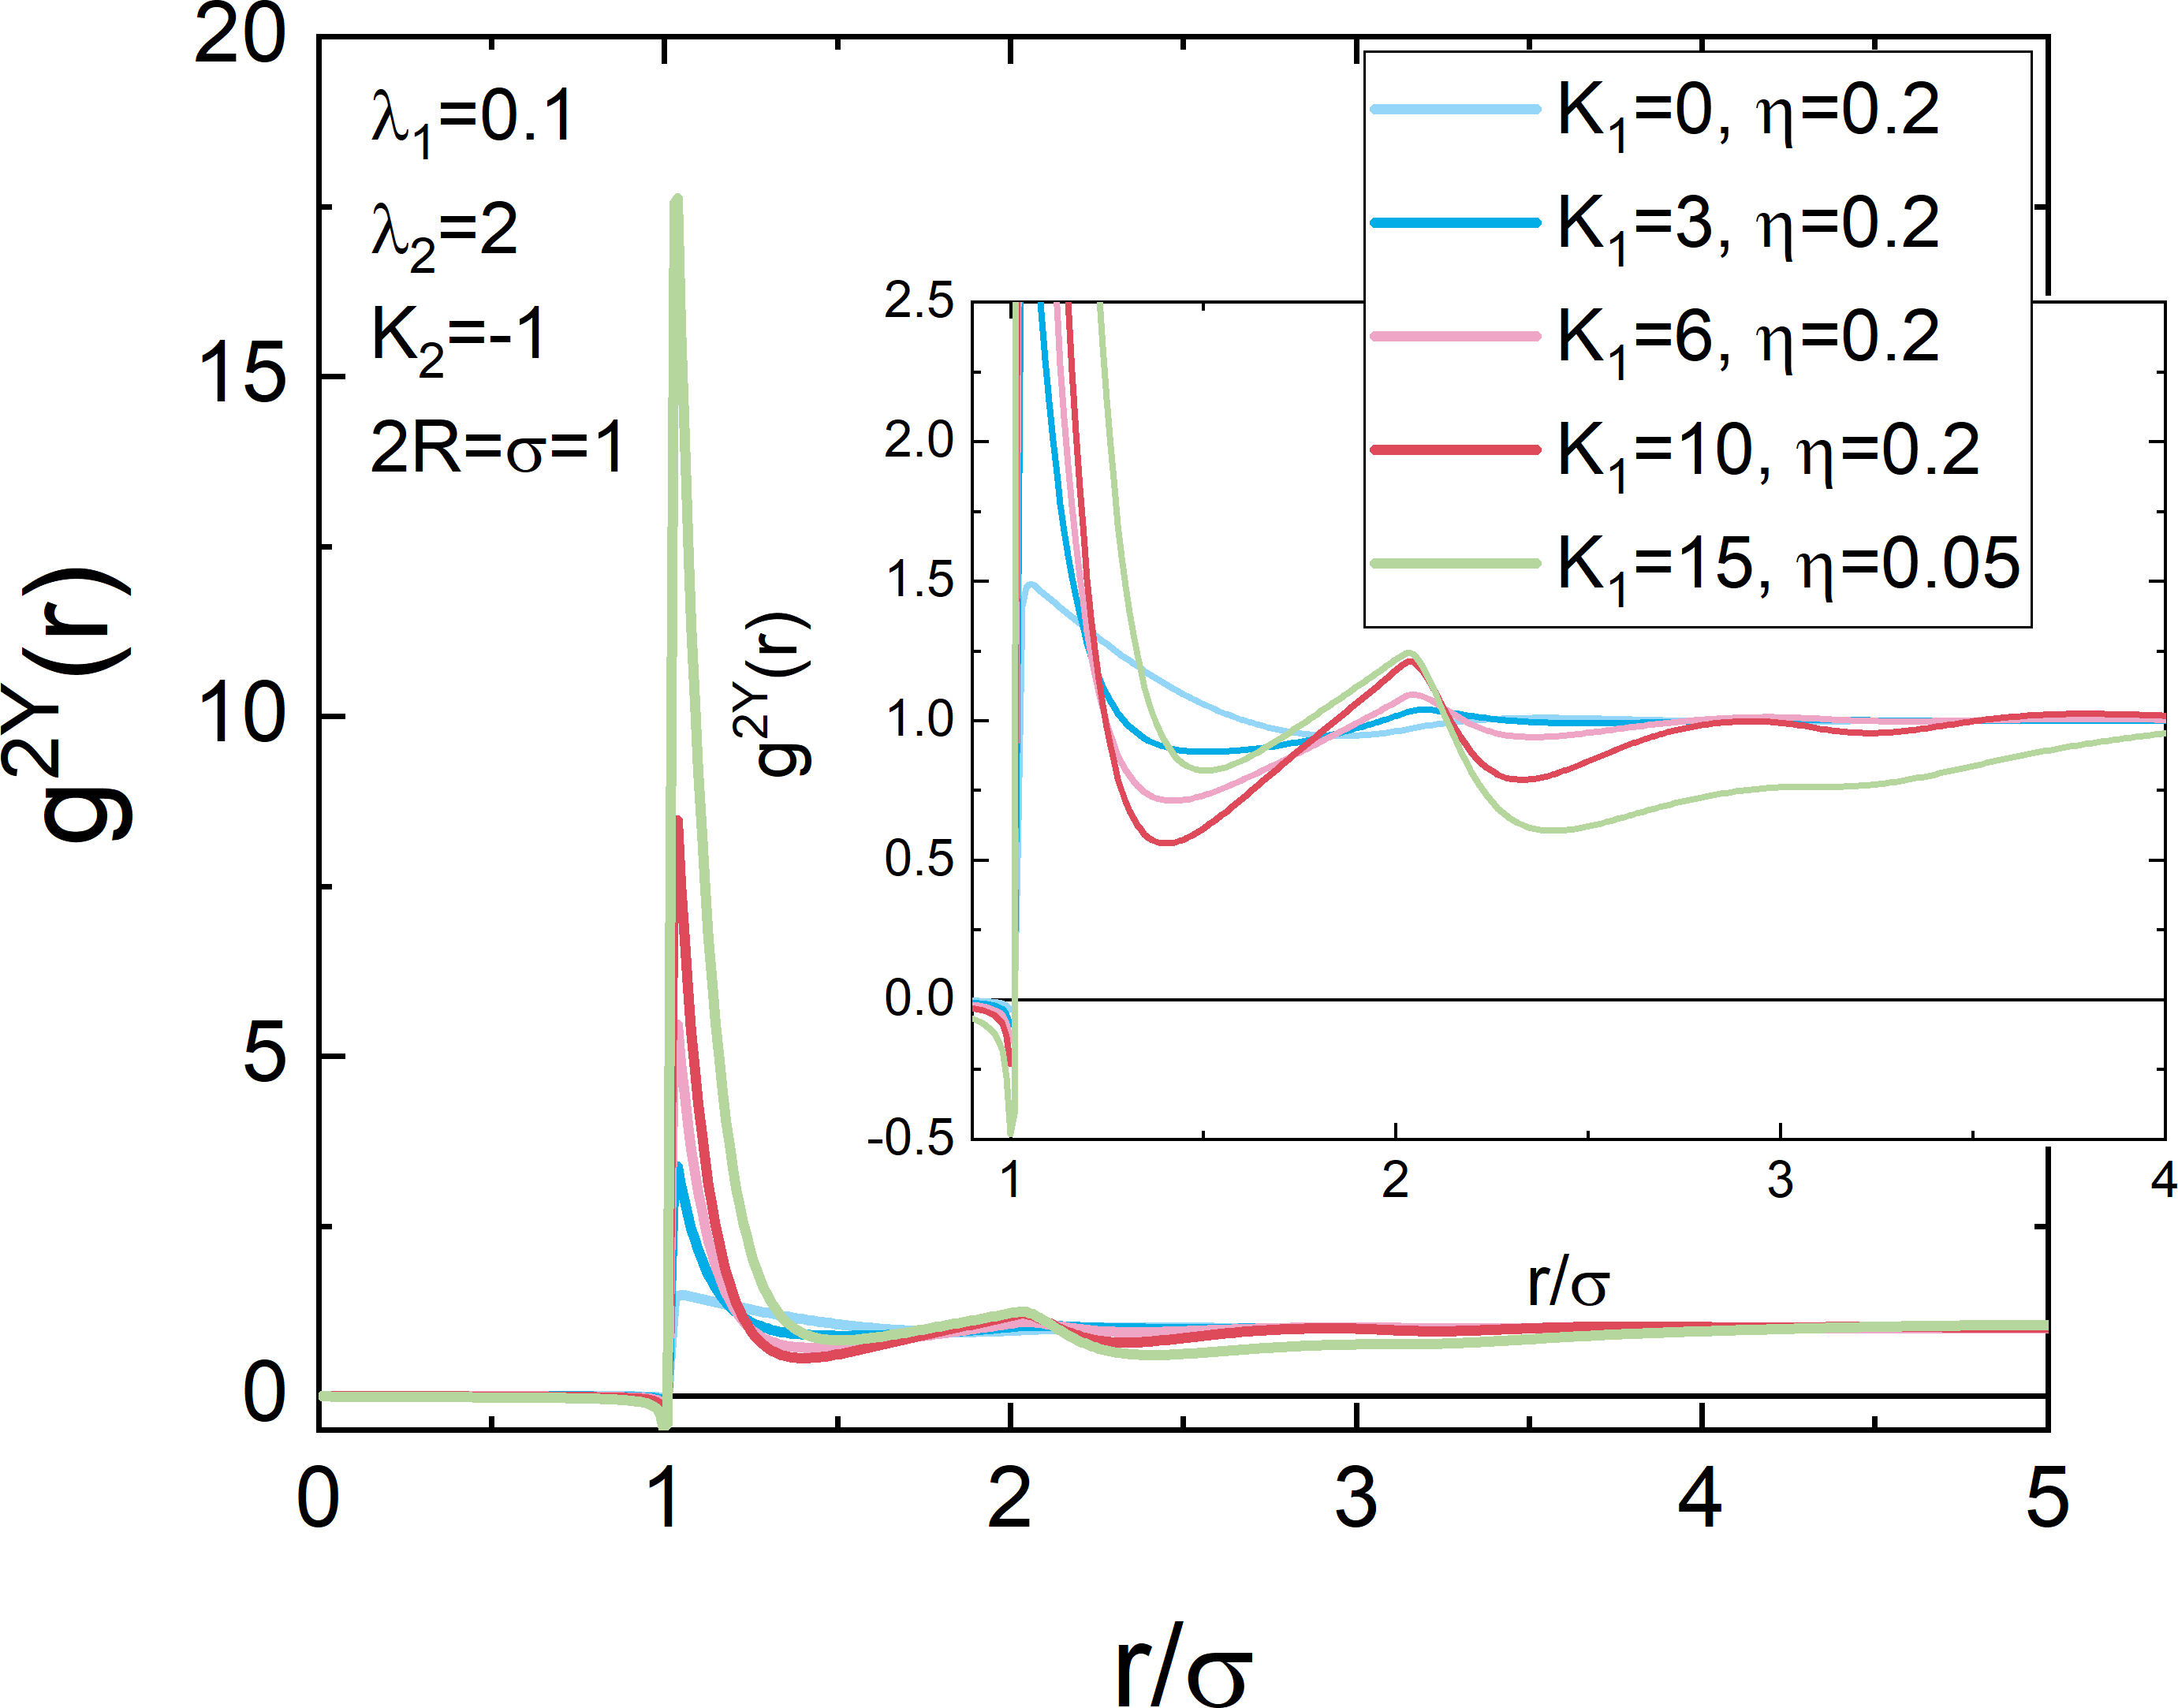
\includegraphics[width=0.48\textwidth]{../images/structure_factor/YukawaLike/TwoYukawa_gr.png}}
\caption{Structure factor radial distribution function for a two-Yukawa potential with an attractive as well as repulsive term.}
\label{fig:Yukawa}
\end{figure}

\noindent\uline{Note:}
\begin{itemize}
  \item The code in \SASfit is based on Matlab code supplied by Yun Liu. The XOP version of this function is based in parts on c-code supplied by Marcus Henning and used for the implementation of this plugin.
  \item For nonphysical or no solution an error message is returned.
  \item For values close to $Z_1=Z_2$ the separately implemented structure factor a single Yukawa interaction potential should be used.
\end{itemize} 

\subsection{Hayter-Penfold structure factor for a screened coulomb interaction (single Yukawa, RMSA)} 

This structure factor has been published in \cite{Hayter1981,Hansen1982}. The original Fortran code has been translates to C by f2c and is used for this plugin.
The repulsive potential used is that one between two identical spherical macroions is given by
\begin{align}\label{eq:HP_RMSA_potential}
  \frac{U_\mathrm{HP}(x)}{k_BT} &= 
  \begin{cases}
    \gamma\frac{\exp(-kx)}{x}, & \mbox{if } x > 1 \\
    \infty, & \mbox{otherwise}.
  \end{cases} \\
  x &= r/\sigma \\
  \sigma &= 2R \\
  k&=\kappa\sigma \\
  K&=q\sigma\\
  k_bT&: \mbox{ thermal energy}\\
  \gamma &=\frac{\pi\epsilon_0\epsilon\sigma}{k_BT}\Psi_0^2  \exp(k) \mbox{ dimensionless coupling constant} \\
  \gamma \exp(-k) & \mbox{  contact potential for macroion pair in unit of $k_B T$}
  \Psi_0 &= z e/(\pi\epsilon\epsilon_0 R(2+\kappa R)) \mbox{surface potential of the particle} \\
  \kappa&=1/\lambda \mbox{ inverse screening length with } \kappa^2=4\pi\lambda_B\sum_i n_iz_i\\
  \lambda_B&= \frac{e^2}{4\pi\epsilon_0\epsilon_r k_BT} \mbox{ Bjerrum length}
\end{align} 
with  $e$ being the elementary charge, $\epsilon_r$ relative dielectric constant of the medium, $\epsilon_0$ is the vacuum permittivity, $n_i$ number density of ion $i$ with charge $z_i$ in units of $e$. 